\newpage
\section{分离变量法}
\subsection{齐次方程}
\begin{ex}[热传导方程]
解热传导方程:
$$\left\{\begin{aligned}
  &\frac{\partial u}{\partial t}=\kappa\frac{\partial^2 u}{\partial t^2}\\
  &u|_{x=0}=u|_{x=l}=0,u|_{t=0}=\phi(x)
\end{aligned}\right.$$

\noindent\textbf{1. 分离变量}

      假设有$u(x,t)=X(x)T(t)$满足PDE和边界条件,暂时不考虑初始条件。
      
      代入方程得到
      $$X(x)T'(t)=\kappa X''(x)T(t)\Rightarrow\frac{T'(t)}{\kappa T(t)}=\frac{X''(x)}{X(x)}=-\lambda$$
     
      (左边不依赖于x,右边不依赖于t,所以都不依赖,为常数)
      
      转换为两个ODE问题:
      $$X''(x)+\lambda X(x)=0, T'(t)+\lambda\kappa T(t)=0$$
      
      边界条件:
      $$u|_{x=0}=X(0)T(t)=0\Rightarrow X(0)=0$$
      $$u|_{x=l}=X(l)T(t)=0\Rightarrow X(l)=0$$

\noindent\textbf{2. 本征值问题}
    $$\left\{\begin{aligned}
        &X''(x)+\lambda X(x)=0\\
        &X(0)=X(l)=0
    \end{aligned}\right.$$

      由Sturm-Liouville Theory可知: $\lambda$为实数

    \noindent i. $\lambda=0$
      $$X(x)=Ax+B$$
      \indent $X(0)=X(l)=0\Rightarrow\quad A=B=0$,无解

    \noindent ii. $\lambda<0$
      $$ X''-|\lambda|X=0\Rightarrow X=Ae^{\sqrt{|\lambda|}x}+Be^{-\sqrt{|\lambda|}x}$$$$X(0)=0=A+B\\ X(l)=0=Ae^{\sqrt{|\lambda|}l}+Be^{-\sqrt{|\lambda|}l}$$
      
      无解
      
    \noindent iii. $\lambda>0$
    $$X=A\sin{\sqrt{\lambda}x}+B\cos{\sqrt{\lambda}x}$$
    $$X(0)=0\Rightarrow B=0\Rightarrow \quad X=A\sin{\sqrt{\lambda}x}\\ X(l)=0\Rightarrow\sqrt{\lambda}l=nπ,\  n=1,2,3,...$$
    
    本征值$\lambda_n=\left(\frac{n\pi}{l}\right)^2$

    本征函数$X_n=\sin\frac{n\pi x}{l}$


\noindent\textbf{3.乘积型解}
      $$T'(t)+\lambda\kappa T(t)=0$$
      $$T'_n(t)+\lambda_n\kappa T_n(t)\Rightarrow T_n(t)=Be^{-\lambda_n\kappa t}=Be^{-\kappa(\frac{nπ}{l})^2t}$$
  $$u_n(x,t)=X_n(x)T_n(t)=B\sin{\frac{nπx}{l}}e^{-\kappa(\frac{nπ}{l})^2t}$$
      此时的$u_n|_{t=0}=B\sin{\frac{nπx}{l}}$

\noindent\textbf{4. 完整解}

    如果初始条件为若干$B\sin{\frac{nπx}{l}}$的和形式,可以马上得到$B_n$和$n$的值,即可通过叠加原理求得$u(t)$

  $$u|_{t=0}=\sum^M_{n=1}B_n\sin{\frac{nπx}{l}}\\\Rightarrow u(x,t)=\sum^M_{n=1}B_n\sin{\frac{nπx}{l}}e^{-\kappa(\frac{nπ}{l})^2t}$$
    “任意”函数$u|_{t=0}=\phi(x)$可展开为
    $$\phi(x)=\sum^{\infty}_{n=1}B_n\sin{\frac{nπx}{l}}=\sum^{\infty}_{n=1}B_nX_n(x)$$,$$X_n=\sin\frac{n\pi}{l}x$$
    求解$B_n$:利用正交性
    
    $\int_0^lX_n(x)X_m(x)dx=0,n\ne m$
    两边同乘$X_n(x)$积分:$$\int_0^l\phi(x)X_n(x)dx=B_n\int_0^l[X_n(x)]^2dx$$
    $$||X_n||^2\equiv\int_0^l[X_n(x)]^2dx=\int_0^l\sin^2\frac{n\pi x}{l}dx=\frac{l}{2}$$
  
    完整解
  $$u(x,t)=\sum^\infty_{n=1}B_n\sin{\frac{nπx}{l}}e^{-\kappa(\frac{nπ}{l})^2t}$$
  
  其中, $$B_n=\frac{1}{||X_n||^2}\int_0^l\phi(x)X_n(x)dx=\frac{2}{l}\int_0^l\phi(x)\sin\frac{n\pi}{l}xdx$$

\end{ex}

\begin{ex}[波动方程:第一、二类边界条件]
    $$\left\{\begin{aligned}
        &\frac{\partial^2{u}}{\partial{t}^2}-a^2\frac{\partial^2{u}}{\partial{x}^2}=0,0<x<l,t>0\\
        &u|_{x=0}=u|_{x=l}=0,\quad u|_{t=0}=\phi(x),\quad\frac{\partial u}{\partial t}\bigg|_{t=0}=\psi(x)
    \end{aligned}\right.$$

   \noindent\textbf{1. 分离变量}
            $$u(x,t)=X(x)T(t)$$
            $$XT''=a^2X''T\Rightarrow\frac{T''(t)}{a^2 T(t)}=\frac{X''(x)}{X(x)}=-\lambda$$
            $$\left\{
        \begin{aligned}
        &X''(x)+\lambda X(x)=0\\
        &T''(t)+\lambda a^2T(t)=0\\
        &X(0)=X(l)=0
                \end{aligned}
        \right.$$
    
    \noindent\textbf{2. 本征值问题}
    
            本征值$$\lambda_n=\left(\frac{n\pi}{l}\right)^2$$

            本征函数$$X_n=\sin\frac{n\pi x}{l}$$

    \noindent\textbf{3.乘积型解}
            $$T''_n(t)+\left(\frac{n\pi a}{l}\right)^2T_n(t)=0$$
            $$T_n(t)=C_n\sin\frac{n\pi a}{l}t+D_n\cos\frac{n\pi a}{l}t$$
            $$u_n(x,t)=X_n(x)T_n(t)=\left(C_n\sin\frac{n\pi a}{l}t+D_n\cos\frac{n\pi a}{l}t\right)\sin\frac{n\pi x}{l}$$
    \noindent\textbf{4. 完整解}
        $$u(x,t)=\sum^\infty_{n=1}\left(C_n\sin\frac{n\pi a}{l}t+D_n\cos\frac{n\pi a}{l}t\right)\sin\frac{n\pi x}{l}$$
          $$\left\{
        \begin{aligned}
        &u|_{t=0}=\phi(x)=\sum_{n=1}^\infty D_n\sin\frac{n\pi x}{l}\\
        &\frac{\partial u}{\partial t}\bigg|_{t=0}=\psi(x)=\sum_{n=1}^\infty C_n\frac{n\pi a}{l}\sin\frac{n\pi x}{l}
                \end{aligned}
        \right.$$
        $$\left\{
        \begin{aligned}
        &D_n=\frac{2}{l}\int_0^l\phi(x)\sin\frac{n\pi x}{l}dx\\
        &C_n=\frac{2}{n\pi a}\int_0^l\psi(x)\sin\frac{n\pi x}{l}dx
                \end{aligned}
        \right.$$
\end{ex}

\begin{ex}[波动方程:第三类边界条件]
    $$\left\{
        \begin{aligned}
        &\frac{\partial^2{u}}{\partial{t}^2}-a^2\frac{\partial^2{u}}{\partial{x}^2}=0,0<x<l,t>0\\
        &u|_{x=0}=0,\quad\left(\frac{\partial u}{\partial x}+hu\right)_{x=l}=0\\
        &u|_{t=0}=\phi(x),
        \quad\frac{\partial u}{\partial t}\bigg|_{t=0}=\psi(x)
                \end{aligned}
        \right.$$
\noindent\textbf{1. 分离变量}
            $$u(x,t)=X(x)T(t)$$
            $$XT''=a^2X''T\Rightarrow\frac{T''(t)}{a^2 T(t)}=\frac{X''(x)}{X(x)}=-\lambda$$
            $$\left\{
        \begin{aligned}
        &X''(x)+\lambda X(x)=0\\
        &T''(t)+\lambda a^2T(t)=0
                \end{aligned}
        \right.$$
            $$u|_{x=0}=0\Rightarrow X(0)=0$$
            $$\left(\frac{\partial u}{\partial x}+hu\right)_{x=l}=[X'(l)+hX(l)]T(t)=0\Rightarrow X'(l)+hX(l)=0$$
\noindent\textbf{2. 本征值问题}
            $$\left\{
        \begin{aligned}
        &X''(x)+\lambda X(x)=0\\
        &X(0)=0\\
        &X'(l)+hX(l)=0
                \end{aligned}
        \right.$$
            Sturm-Liouville Theory: $\lambda$为实数

            \noindent i. $\lambda=0$,无解

            \noindent ii. $\lambda<0$,无解

            \noindent iii. $\lambda>0$
            $$X=A\sin{\sqrt{\lambda}x}+B\cos{\sqrt{\lambda}x}$$
            $$X(0)=0\Rightarrow B=0\Rightarrow \quad X=A\sin{\sqrt{\lambda}x}\\ X'(l)+hX(l)=A(\sqrt{\lambda}\cos\sqrt{\lambda}l+h\sin\sqrt{\lambda}l)=0$$
            $$\tan(\sqrt{\lambda}l)=-\frac{\sqrt{\lambda}}{h}$$
              记$\sqrt{\lambda}l=\mu$,有$\tan\mu=-\frac{\mu}{hl}$
              $$\lambda_n=\left(\frac{\mu_n}{l}\right)^2$$
              $$X_n=\sin{\sqrt{\lambda_n}x}=\sin{\frac{\mu_nx}{l}}$$
\noindent\textbf{3.乘积型解}
            $$T''_n(t)+\lambda_na^2T_n(t)=0$$
            $$T_n(t)=C_n\sin\sqrt{\lambda_n}at+D_n\cos\sqrt{\lambda_n}at$$
            $$u_n(x,t)=X_n(x)T_n(t)=\left(C_n\sin\sqrt{\lambda_n}at+D_n\cos\sqrt{\lambda_n}at\right)\sin{\sqrt{\lambda_n}x}$$
\noindent\textbf{4. 完整解}

          仍然有正交性$$\int_0^lX_n(x)X_m(x)dx=0,n\ne m$$
        $$||X_n||^2\equiv\int_0^l[X_n(x)]^2dx=\int_0^l\frac{1-\cos(2\sqrt{\lambda_n}x)}{2}dx=\frac{l}{2}\left[1-\frac{\sin(2\sqrt{\lambda_n}l)}{2\sqrt{\lambda_n}l}\right]$$
          $$u|_{t=0}=\phi(x)=\sum_{n=1}^\infty D_n\sin{\sqrt{\lambda_n}x}$$
          $$\frac{\partial u}{\partial t}\bigg|_{t=0}=\psi(x)=\sum_{n=1}^\infty C_n\sqrt{\lambda_n}a\sin(\sqrt{\lambda_n}x)$$
        $$D_n=\frac{1}{||X_n||^2}\int_0^l\phi(x)\sin(\sqrt{\lambda_n}x)dx$$
        $$C_n=\frac{1}{\sqrt{\lambda_n}a||X_n||^2}\int_0^l\psi(x)\sin(\sqrt{\lambda_n}x)dx$$
\end{ex}

\begin{ex}[Laplace方程]
$$\left\{
\begin{aligned}
&\frac{\partial^2{u}}{\partial{x}^2}+\frac{\partial^2{u}}{\partial{y}^2}=0\\
&u(0,y)=u(a,y)=0,\quad u(x,0)=0,\quad u(x,b)=f(x)
        \end{aligned}
\right.$$
若边界条件为下图所示,则将以下四种边界条件的解叠加。
\begin{figure}[H]
    \centering 
    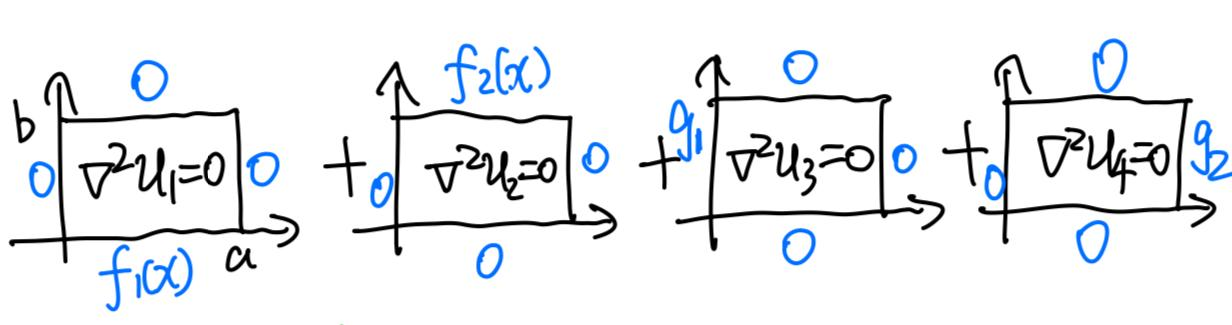
\includegraphics[width=10cm]{figures/Rec_HeatTransfer.JPEG} 
    \label{Rec_HeatTransfer}
\end{figure}
\noindent\textbf{1. 分离变量}
    $$u(x,y)=X(x)Y(y)$$
    $$XY''+X''Y=0\Rightarrow\frac{X''(x)}{ X(x)}=-\frac{Y''(y)}{Y(y)}=-\lambda$$
    $$\left\{
\begin{aligned}
    &X''(x)+\lambda X(x)=0\\
    &Y''(t)-\lambda Y(y)=0\\
    &X(0)=X(a)=0
\end{aligned}
\right.$$
\noindent\textbf{2. 本征值问题}

    本征值$$\lambda_n=\left(\frac{n\pi}{a}\right)^2$$

    本征函数$$X_n=\sin\frac{n\pi x}{a}$$

    \noindent\textbf{3.乘积型解}
    $$Y''_n(y)-\left(\frac{n\pi}{l}\right)^2Y_n(y)=0$$
    $$Y_n(y)=C_n\sinh\frac{n\pi}{a}y+D_n\cosh\frac{n\pi}{a}y$$
    $$u_n(x,y)=X_n(x)Y_n(y)=\left(C_n\sinh\frac{n\pi}{a}y+D_n\cosh\frac{n\pi}{a}y\right)\sin\frac{n\pi x}{a}$$
    \noindent\textbf{4. 完整解}
$$u(x,y)=\sum^\infty_{n=1}\left(C_n\sinh\frac{n\pi}{a}y+D_n\cosh\frac{n\pi}{a}y\right)\sin\frac{n\pi x}{a}$$
  $$u|_{y=0}=\sum_{n=1}^\infty D_n\sin\frac{n\pi x}{a}=0\Rightarrow D_n=0$$
  $$u|_{y=b}=\sum_{n=1}^\infty C_n\sinh\frac{n\pi b}{a}\sin\frac{n\pi x}{a}=f(x)$$
$$u(x,y)=\sum^\infty_{n=1}C_n\sinh\frac{n\pi}{a}y\sin\frac{n\pi x}{a}$$
$$C_n=\frac{2}{a\sinh\frac{n\pi b}{a}}\int_0^af(x)\sin\frac{n\pi x}{a}dx$$
\end{ex}

\subsection{齐次多变量问题}
\begin{ex}[二维扩散问题]
    $$\left\{
        \begin{aligned}
        &
        \frac{\partial{u}}{\partial{t}}=\frac{\partial}{\partial x}\left(D\frac{\partial{u}}{\partial{x}}\right) +\frac{\partial}{\partial y}\left(D\frac{\partial{u}}{\partial{y}}\right)\\
        &\text{绝热边界:}\frac{\partial{u}}{\partial x}\bigg|_{x=0}=\frac{\partial{u}}{\partial x}\bigg|_{x=a}=\frac{\partial{u}}{\partial y}\bigg|_{y=0}=\frac{\partial{u}}{\partial y}\bigg|_{y=b}=0\\
        &u|_{t=0}=\phi(x,y)
                \end{aligned}
        \right.
        $$

\noindent\textbf{1. 分离变量}
$$u(x,y,b)=X(x)Y(y)T(t)$$
$$\frac{1}{D}XYT'=X''YT+XY''T$$
$$\begin{aligned}
&\Rightarrow \frac{X''}{X}+\frac{Y''}{Y}=\frac{1}{D}\frac{T'}{T}=-\lambda\\
&\therefore\frac{X''}{X}=-\mu,\frac{Y''}{Y}=-\nu,\lambda=\mu+\nu
\end{aligned}$$

\noindent\textbf{2. 本征值问题}

$$\left\{
    \begin{aligned}
    &X''+\mu X=0\\
    &X'(0)=X'(a)=0
            \end{aligned}
    \right.$$
\begin{enumerate}
    \item{$\mu=0, X_n(x)=Ax+B\Rightarrow X_0(x)=1$}
    \item{$\mu>0,X_n=\cos{\frac{n\pi x}{a}},\mu_ n=\left(\frac{n\pi}{a}\right)^2,n=1,2,3,...$}
    \item {$\mu<0$,无解}
\end{enumerate}
合并1, 2:$$\mu_ n=\left(\frac{n\pi}{a}\right)^2, X_n=\cos{\frac{n\pi x}{a}}, n=0,1,2,...$$
        $$\left\{
    \begin{aligned}
    &Y''+\nu X=0\\
    &Y'(0)=Y'(b)=0
            \end{aligned}
    \right.$$
同理可得:
        $$Y_m(y)=\cos{\frac{m\pi x}{b}},\nu_ n=\left(\frac{m\pi}{b}\right)^2,n=0,1,2,...$$
        $$\lambda_{mn}=\mu_ n+\nu_ m=\left(\frac{n\pi}{a}\right)^2+\left(\frac{m\pi}{b}\right)^2$$
        
\noindent\textbf{3.乘积型解}
        $$T_{nm}'(t)=-\lambda_{nm}DT(t)$$
        $$\Rightarrow T_{nm}(t)=A_{mn}e^{-\lambda_{nm}Dt}$$
        $$u_{nm}(x,y,t)=X_n(x)Y_m(y)T_{nm}(t)$$
        
\noindent\textbf{4. 完整解}
        $$u(x,y,t)=\sum_{n,m}u_{nm}(x,y,t)=\sum_{n,m=0}^\infty\cos{\frac{n\pi x}{a}}\cos{\frac{m\pi x}{b}}e^{-[\left(\frac{n\pi}{a}\right)^2+\left(\frac{m\pi}{b}\right)^2]t}$$
        二重傅里叶级数(1)
        $$u|_{t=0}=\phi(x,y)=\sum_{n,m=0}^{\infty}A_{nm}\cos{\frac{n\pi x}{a}}\cos{\frac{m\pi x}{b}}$$
        正交性:
    $$\int_0^a{X_nX_{n'}dx}=
    \begin{cases}
    \dfrac{a}{2}& n=n'\ne 0\\
    a&n=n'=0\\
    0& n\ne n'
    \end{cases}
    \equiv\frac{a}{2}(1+\delta_{n0})\delta_{nn'}$$

        同理:$$\int_0^bY_mY_{m'}dy=\frac{b}{2}(1+\delta_{m0})\delta_{mm'}$$
        (1)式两边同乘$X_nY_m$并作积分$\int_0^a\int_0^bdxdy$得:
        $$\int_0^a\int_0^b\phi(x,y)\cos{\frac{n\pi x}{a}}\cos{\frac{m\pi x}{b}}dxdy=\frac{a}{2}(1+\delta_{n0})\frac{b}{2}(1+\delta_{m0})A_{nm}$$
        $$A_{mn}=\frac{4}{ab}\frac{1}{(1+\delta_{n0})(1+\delta_{m0})}\int_0^a\int_0^b\phi(x,y)\cos{\frac{n\pi x}{a}}\cos{\frac{m\pi x}{b}}dxdy$$

\end{ex}

\subsection{非齐次方程}
\subsubsection{齐次化原理}
考虑以下非齐次方程
$$\left\{
\begin{aligned}
&
\frac{\partial^2{u}}{\partial{t}^2}-a^2\frac{\partial^2{u}}{\partial{x}^2}=f(x,t)\quad 0<x<l,t>0\\
&u|_{x=0}=u|_{x=l}=0\\
&u|_{t=0}=\frac{\partial{u}}{\partial t}\bigg|_{t=0}=0
        \end{aligned}
\right.$$

引入辅助函数$w(x,t;\tau)$,满足
$$w(x,t;\tau):\left\{
\begin{aligned}
&
\frac{\partial^2{w}}{\partial{t}^2}-a^2\frac{\partial^2{w}}{\partial{x}^2}=0\quad 0<x<l,t>\tau\\
&w|_{t=\tau}=0,\frac{\partial{w}}{\partial t}\bigg|_{t=\tau}=f(x,\tau)
        \end{aligned}
\right.$$
可以得到方程的解
$$u(x,t)=\int_0^tw(x,t;\tau)d\tau$$
$$w(x,t;\tau)=\sum_{n=1}^{\infty}C_n(\tau)\sin{[\frac{n\pi a}{l}(t-\tau)]}\sin{\frac{n\pi a}{l}}dx$$
其中,
$$C_n=\frac{l}{n\pi a}\frac{2}{l}\int_{0}^{l}f(x,\tau)\sin{\frac{n\pi x}{l}}dx=\frac{l}{n\pi a}f_n(\tau)$$
$$\begin{aligned}
    u(x,t)&=\int_0^tw(x,t;\tau)d\tau\\
    &=\sum_{n=1}^\infty\left[\int^t_0C_n(\tau)\sin{\frac{n\pi a}{l}(t-\tau)}d\tau\right]\sin{\frac{n\pi x}{l}}\\
    &=\sum_{n=1}^\infty\left[\int^t_0\frac{l}{n\pi a}f_n(\tau)\sin{\frac{n\pi a}{l}(t-\tau)}d\tau\right]\sin{\frac{n\pi x}{l}}\\
    &\equiv\sum_{n=1}^\infty T_n(t)X_n(x)
    \end{aligned}$$

\subsubsection{本征函数展开法}
根据齐次化原理的结果,提示解取此形式分离变量:
$$u(x,t)=\sum_{n=1}^\infty T_n(t)X_n(x)$$

展开$f(x,t)$
$$f(x,t)=\sum_{n=1}^\infty f_n(t)X_n(x)$$
$$\frac{\partial^2{u}}{\partial{t}^2}-a^2\frac{\partial^2{u}}{\partial{x}^2}=f(x,t)\Rightarrow \sum_{n=1}^\infty T_n''X_n-a^2T_nX_n''=\sum_{n=1}^\infty f_nX_n$$

又$X_n''=-\lambda_nX_n$
$$\sum_{n=1}^\infty(T_n''+a^2\lambda_nT_n-f_n)X_n=0$$
$$T_n''(t)+a^2\lambda_nT_n(t)=f_n(t), \lambda_n=\left(\frac{n\pi}{l}\right)^2$$

化为解非齐次ODE问题:$$T_n''(t)+\left(\frac{n\pi a}{l}\right)^2T_n(t)=f_n(t)$$
$$W(t;\tau):\left\{
\begin{aligned}
&
W_n''+\left(\frac{n\pi a}{l}\right)^2W_n=0\\
&W|_{t=\tau}=0,W_n'|_{t=\tau}=f_n(\tau)
        \end{aligned}
\right.$$
$$T(x,t)=\int_0^tW(t;\tau)d\tau$$
$$W_n=(t,\tau)=f_n(\tau)\frac{l}{n\pi a}\sin\frac{n\pi a}{l}(t-\tau)$$
$$T(t)=\int_0^tW(t;\tau)d\tau=\frac{l}{n\pi a}\int_0^tf_n(\tau)\sin\frac{n\pi a}{l}(t-\tau)d\tau$$
$$u(x,t)=\sum_{n=1}^\infty T_n(t)X_n(x)$$

\subsubsection{特解法}
找特解$v$满足:$$\frac{\partial^2{v}}{\partial{t}^2}-a^2\frac{\partial^2{v}}{\partial{x}^2}=f(x,t), v|_{x=0}=v|_{x=l}=0$$

$u(x,t)=v(x,t)$(已取定)$+w(x,t)$(待求)
$$\frac{\partial^2{(v+w)}}{\partial{t}^2}-a^2\frac{\partial^2{(v+w)}}{\partial{x}^2}=f(x,t)$$
$$\Rightarrow \frac{\partial^2{w}}{\partial{t}^2}-a^2\frac{\partial^2{w}}{\partial{x}^2}=0, w|_{x=0}=w|_{x=l}=0$$

\subsection{非齐次边界条件}
\subsubsection{边界条件齐次化}
$$\left\{
    \begin{aligned}
    &
    \frac{\partial^2{u}}{\partial{t}^2}-a^2\frac{\partial^2{u}}{\partial{x}^2}=f(x,t)\quad 0<x<l,t>0\\
    &u|_{x=0}=\mu(t),u|_{x=l}=\nu(t)\\
    &u|_{t=0}=\phi(x),\frac{\partial{u}}{\partial t}\bigg|_{t=0}=\psi(x)
            \end{aligned}
    \right.$$
\noindent\textbf{Step 1 边界条件齐次化}
$$u(x,t)=p(x,t)+w(x,t)$$
$$p|_{x=0}=\mu(t),p|_{x=l}=\nu(t)$$

$p$满足边界条件,但不必满足PDE
$$\Rightarrow w|_{x=0}=u|_{x=0}-p|_{x=0}=0,w|_{x=l}=0$$
\noindent\textbf{Step 2 求解$w(x,t)$}
$$\frac{\partial^2{w}}{\partial{t}^2}-a^2\frac{\partial^2{w}}{\partial{x}^2}=\frac{\partial^2{(u-p)}}{\partial{t}^2}-a^2\frac{\partial^2{(u-p)}}{\partial{x}^2}=f(x,t)-\left(\frac{\partial^2{p}}{\partial{t}^2}-a^2\frac{\partial^2{p}}{\partial{x}^2}\right)$$
$$w|_{x=0}=w|_{x=l}=0$$
$$w|_{t=0}=u|_{t=0}-p|_{t=0}=\phi(x)-p|_{t=0}$$
$$\frac{\partial{w}}{\partial t}\bigg|_{t=0}=\frac{\partial{u}}{\partial t}\bigg|_{t=0}-\frac{\partial{p}}{\partial t}\bigg|_{t=0}=\psi(x)-\frac{\partial{p}}{\partial t}\bigg|_{t=0}$$

\noindent\textbf{$p$的选取:自由度较大}

\textbf{第一类:}边界上的函数值$u|_{x=0}=\mu(t),u|_{x=l}=\nu(t)$
    $$p(x,t)=A(t)x+B(t)=\mu(t)+\frac{\nu(t)-\mu(t)}{l}x$$
    $$p(x,t)=A(t)(l-x)^2+B(t)x^2=\frac{\mu(t)}{l^2}(l-x)^2+\frac{\nu(t)}{l}x^2$$

    \textbf{第二类:}边界上的函数微商$\frac{\partial{u}}{\partial x}|_{x=0}=\mu(x),\frac{\partial{u}}{\partial x}|_{x=l}=\nu(x)$
    $$p(x,t)=A(t)x^2+B(t)x=\left(\frac{\nu(t)}{2l}-\frac{\mu(t)}{2}\right)x^2+\mu(t)x$$
    
    \textbf{第三类:}混合边界条件,指定边界上函数值与微商的线性关系
    $$\alpha_1u+\beta_1\frac{\partial{u}}{\partial x}\big|_{x=0}=\mu(x),\alpha_2u+\beta_2\frac{\partial{u}}{\partial x}\big|_{x=l}=\nu(x)$$
    $$p(x,t)=A(t)x^2+B(t)$$
    $$\left( \begin{array}{ccc}
        \beta_1 & \alpha_1 \\
        \alpha_2l+\beta_2 & \alpha_2 
        \end{array} 
        \right )
        \left( \begin{array}{ccc}
        A(t) \\
        B(t)
        \end{array} 
        \right )
        =
        \left( \begin{array}{ccc}
        \mu(t) \\
        \nu(t)
        \end{array} 
    \right )$$
    
    $$\left( \begin{array}{ccc}
        A(t) \\
        B(t)
        \end{array} 
        \right )
        =\frac{1}{\beta_1\alpha_2-\alpha_1\beta_2-\alpha_1\alpha_2l}\left( \begin{array}{ccc}
        \alpha_2 & -\alpha_1 \\
        -(\alpha_2l+\beta_2) & \beta_1
        \end{array} 
        \right )
        \left( \begin{array}{ccc}
        \mu(t) \\
        \nu(t)
            \end{array} 
    \right )$$

\begin{ex}[弦受迫振动]
    $$\left\{
        \begin{aligned}
        &
        \frac{\partial^2{u}}{\partial{t}^2}-a^2\frac{\partial^2{u}}{\partial{x}^2}=0\quad 0<x<l,t>0\\
        &u|_{x=0}=0,u|_{x=l}=A\sin\omega t\\
        &u|_{t=0}=0,\frac{\partial{u}}{\partial t}\bigg|_{t=0}=0
                \end{aligned}
        \right.$$
\end{ex}

$$p(x,t)=\mu(t)+\frac{\nu(t)-\mu(t)}{l}x=\frac{Ax}{l}\sin\omega t$$
$$\frac{\partial^2{w}}{\partial{t}^2}-a^2\frac{\partial^2{w}}{\partial{x}^2}=-\left(\frac{\partial^2{p}}{\partial{t}^2}-a^2\frac{\partial^2{p}}{\partial{x}^2}\right)=\frac{A\omega^2x}{l}\sin\omega t$$
$$w|_{x=0}=w|_{x=l}=0$$
$$w|_{t=0}=-p|_{t=0}=0$$
$$\frac{\partial{w}}{\partial t}\bigg|_{t=0}=-\frac{\partial{p}}{\partial t}\bigg|_{t=0}=-\frac{A\omega}{l}x$$ 
$$w=w_1+w_2$$
$$w_1:\left\{
\begin{aligned}
&
\frac{\partial^2{w_1}}{\partial{t}^2}-a^2\frac{\partial^2{w_1}}{\partial{x}^2}=0\\
&w_1|_{x=0}=w_1|_{x=l}=0\\
&w_1|_{t=0}=0,\frac{\partial{w_1}}{\partial t}\bigg|_{t=0}=-\frac{A\omega}{l}x
    \end{aligned}
\right.\quad w_2:\left\{
\begin{aligned}
&
\frac{\partial^2{w_2}}{\partial{t}^2}-a^2\frac{\partial^2{w_2}}{\partial{x}^2}=\frac{A\omega^2x}{l}\sin\omega t\\
&w_2|_{x=0}=w_2|_{x=l}=0\\
&w_2|_{t=0}=\frac{\partial{w_2}}{\partial t}\bigg|_{t=0}=0
    \end{aligned}
\right.$$

\noindent 解1:
$$w_1=\sum_{n=1}^\infty C_n\sin\omega_nt\sin\frac{n\pi x}{l}, \omega_n=\frac{n\pi a}{l}$$
$$\frac{\partial{w_1}}{\partial t}\bigg|_{t=0}=\sum_{n=1}^\infty C_n\omega_n\sin\frac{n\pi x}{l}-\frac{A\omega}{l}x\Rightarrow C_n=(-1)^n\frac{2A\omega}{n\pi\omega_n}$$
\noindent 解2:
$$w_2=\sum^\infty_{n=1}\frac{g_n}{\omega_n}\frac{\omega\sin{\omega_nt}-\omega_n\sin\omega t}{\omega^2-\omega_n^2}\sin\frac{n\pi x}{l}$$
Where $$g_n=\frac{2}{l}\int_0^lg(x)\sin\frac{n\pi x}{l}dx=\frac{2A\omega^2}{n\pi}(-1)^{n+1}$$
$$w=w_1+w_2=\sum_{n=1}^\infty(-1)^{n}\frac{2Aa}{l}\frac{\omega_n\sin\omega t-\omega\sin\omega_nt}{\omega^2-\omega_n^2}\sin\frac{n\pi x}{l}$$


\begin{ex}[温度周期边界条件]
$$\left\{
    \begin{aligned}
        &\frac{\partial{u}}{\partial{t}}-D\frac{\partial^2{u}}{\partial{x}^2}=0\quad 0<x<l,t>0\\
        &u|_{x=0}=A\sin\omega t, u|_{x=l}=0\\
        &u|_{t=0}=0
    \end{aligned}
\right.$$
$$p(x,t)=\mu(t)+\frac{v(t)-\mu(t)}{l}x=A(1-\frac{x}{l}\sin\omega t)$$
$$\left\{
    \begin{aligned}
        &\frac{\partial{w}}{\partial{t}}-D\frac{\partial^2{w}}{\partial{x}^2}=-\left(\frac{\partial{p}}{\partial{t}}-D\frac{\partial^2{p}}{\partial{x}^2}\right)=-A\omega(1-\frac{x}{l})\cos\omega t\quad 0<x<l,t>0\\
        &w|_{x=0}=w|_{x=l}=0\\
        &w|_{t=0}=-p|_{t=0}=0
     \end{aligned}
\right.$$

齐次化原理:
$$w(x,t)=\int_0^tv(x,t;\tau)d\tau,v|_{t=\tau}=f(x,\tau)=\sum_{n=1}^\infty f_n(\tau)\sin{\frac{n\pi x}{l}}$$
$$w(x,t)=\int_0^tv(x,t;\tau)d\tau=\sum_{n=1}^\infty\left[f_n(\tau)e^{-D(\frac{n\pi}{l})^2(t-\tau)}d\tau\right]\sin\frac{n\pi x}{l}$$
$$f_n(\tau)=\frac{2}{l}\int_0^lf(x,\tau)\sin\frac{n\pi x}{l}dx=-\frac{2A\omega}{n\pi}\cos\omega t$$

得到
$$w(x,t)=\sum_{n=1}^\infty\frac{2A\omega l^2}{D^2(n\pi)^4+\omega^2l^4}\frac{1}{n\pi}\left[D(n\pi)^2e^{-D(\frac{n\pi}{l})^2t}-D(n\pi)^2\cos\omega t-\omega l^2\sin\omega t\right]\sin\frac{n\pi x}{l}$$
$$u=p+w$$
\end{ex}
\subsubsection{方程与边界条件同时齐次化}

\begin{ex}
$$\left\{\begin{aligned}
&\frac{\partial^2{u}}{\partial{t}^2}-a^2\frac{\partial^2{u}}{\partial{x}^2}=0\quad 0<x<l,t>0\\
&u|_{x=0}=0,u|_{x=l}=A\sin\omega t\\
&u|_{t=0}=0,\frac{\partial{u}}{\partial t}\bigg|_{t=0}=0
\end{aligned}\right.$$
    $$u=p+w$$

    $p$不仅满足边界条件,还满足方程:
$$\left\{
\begin{aligned}
&\frac{\partial^2{p}}{\partial{t}^2}-a^2\frac{\partial^2{p}}{\partial{x}^2}=0\quad 0<x<l,t>0\\
&p|_{x=0}=0,p|_{x=l}=A\sin\omega t
\end{aligned}\right.$$

    设$p(x,t)=f(x)\sin\omega t, f(0)=0,f(l)=A$
    $$[\omega^2f(x)+a^2f''(x)]\sin\omega t=0\Rightarrow f(x)=A\frac{\sin\frac{\omega x}{a}}{\sin\frac{\omega l}{a}}$$
    $$p(x,t)=A\frac{\sin\frac{\omega x}{a}}{\sin\frac{\omega l}{a}}\sin\omega t$$

    $$\left\{\begin{aligned}
&\frac{\partial^2{w}}{\partial{t}^2}-a^2\frac{\partial^2{w}}{\partial{x}^2}=0\quad 0<x<l,t>0\\
&w|_{x=0}=w|_{x=l}=0\\
&w|_{t=0}=-p|_{t=0}=0,\frac{\partial{w}}{\partial t}\bigg|_{t=0}=-\frac{\partial{p}}{\partial t}\bigg|_{t=0}=-A\frac{\sin\frac{\omega x}{a}}{\sin\frac{\omega l}{a}}
\end{aligned}\right.$$
    $$w(x,t)=\sum_{n=1}^\infty(-1)^{n+1}\frac{2Aa\omega}{l(\omega^2-\omega_n^2)}\sin\omega_n t\sin\frac{n\pi x}{l}$$
    $$p(x,t)=A\frac{\sin\frac{\omega x}{a}}{\sin\frac{\omega l}{a}}\sin\omega t=\sum_{n=1}^\infty(-1)^{n}\frac{2Aa\omega_n}{l}\frac{1}{\omega^2-\omega_n^2}\sin\omega t\sin\frac{n\pi x}{l}$$
    $$u=p+w=\sum_{n=1}^\infty(-1)^{n}\frac{2Aa}{l}\frac{\omega_n\sin\omega t-\omega\sin\omega_nt}{\omega^2-\omega_n^2}\sin\frac{n\pi x}{l}$$

\end{ex}
